\documentclass[10pt]{article}
\usepackage[letterpaper,margin=1in]{geometry}
\usepackage{lmodern}
\usepackage[T1]{fontenc}
\usepackage{amsmath,amssymb}
\usepackage{booktabs}
\usepackage{tikz}
\usetikzlibrary{arrows.meta,positioning}
\usepackage[colorlinks=true,linkcolor=black,citecolor=black,urlcolor=blue]{hyperref}
\usepackage{caption}
\captionsetup{font=small,labelfont=bf}
\setlength{\parskip}{4pt}
\setlength{\parindent}{0pt}

\definecolor{trade}{HTML}{1F4FA3}
\definecolor{info}{HTML}{6A48C0}
\definecolor{repair}{HTML}{A8630F}
\definecolor{neutral}{HTML}{6B7280}

\begin{document}

\begin{center}
\rule{\textwidth}{2pt}\\[8pt]
{\LARGE\bfseries MarketDebug: Paying Gemma Agents for What They Find}\\[6pt]
{\large Prediction markets, information rewards and repair bounties for small-model fault localization}\\[6pt]
\rule{\textwidth}{0.5pt}\\[12pt]
\begin{tabular}{cccc}
\textbf{Aarush Aggarwal} & \textbf{Ratul Chakraborty} & \textbf{Raunak Mondal} & \textbf{Aarush Raheja}
\end{tabular}\\[4pt]

\end{center}

\vspace{6pt}
\begin{center}\textbf{Abstract}\end{center}
\begin{quote}\small
Multi-agent coding systems usually combine agents by voting or by concatenating their outputs. Neither gives an agent a reason to search for evidence the others missed. We present MarketDebug, a mechanism that gives each agent capital and positions in logarithmic market scoring rule (LMSR) prediction markets about where a bug is. Rewards come from three separate ledgers: trading profit for being right early, Shapley information rewards for evidence that improves the group forecast, and a repair bounty for a passing patch. We evaluate the market layer on MarketBugs, a held-out set of 210 single-function bugs from seven Python repositories. Five Gemma~4 E4B specialists act as traders, and their beliefs are frozen Gemma forecasts. The market matches the strongest baseline on top-1 localization (64.3\% vs.\ 64.8\%; paired difference $-0.5$ pp, 95\% repository-cluster CI $[-4.8, +3.8]$). It reduces log loss on the gold function from 1.40 to 1.06 nats. Exact Shapley credit identifies the specialists whose evidence matters. Markets are therefore a practical way to obtain calibrated forecasts from small local models, but they do not by themselves find more bugs.
\end{quote}

\section{Introduction}
Small open models that run on one accelerator are weak at multi-step software engineering. A common response is to run several instances and aggregate them. When every instance is the same small model, aggregation has little independent signal to work with. Prior work on MarketBugs found exactly this: a learned pool of five Gemma specialists was statistically indistinguishable from a single call that saw all five notes~\cite{marketbugs}.

Aggregation without incentives is a poll. We ask a different question: \emph{what if each agent were paid for information the group does not yet have?} Markets do this for people. A trader profits only by disagreeing with the price and being right. Conitzer showed how scoring rules and cooperative game theory can reward the contribution of information itself~\cite{conitzer2009}, and Hanson's LMSR provides liquidity even with few traders~\cite{hanson2003}.

Our contributions:
\begin{itemize}\setlength{\itemsep}{1pt}
\item \textbf{A three-ledger incentive design} for debugging agents. It separates trading rewards, information rewards and repair rewards, so that no single behavior can be gamed for all three (Section~\ref{sec:method}).
\item \textbf{An open implementation}: LMSR markets, an evidence board that refuses credit to copied facts, marginal, Shapley and pivotal information rewards, and test-ordered patch settlement, with a common agent interface for simulated or Gemma agents.
\item \textbf{An evaluation on real Gemma~4 E4B forecasts} over 240 MarketBugs bugs. The market improves calibration substantially without changing accuracy, and exact Shapley values rank the specialists consistently with their standalone usefulness (Section~\ref{sec:exp}).
\end{itemize}

\begin{figure}[t]
\centering
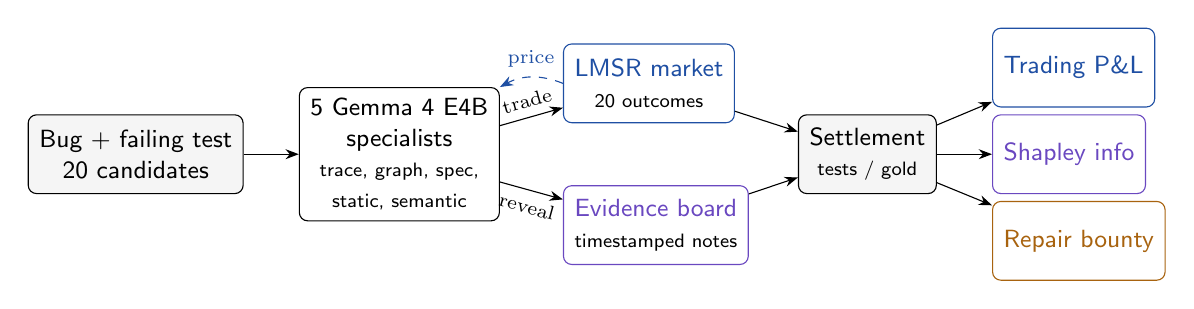
\begin{tikzpicture}[font=\sffamily\small, box/.style={draw, rounded corners=3pt, align=center, minimum height=1.0cm, inner sep=4pt}, >=Stealth]
\node[box, fill=gray!8] (repo) {Bug + failing test\\20 candidates};
\node[box, right=0.7cm of repo] (agents) {5 Gemma 4 E4B\\specialists\\{\scriptsize trace, graph, spec,}\\{\scriptsize static, semantic}};
\node[box, draw=trade, right=0.8cm of agents, yshift=0.9cm] (mkt) {\textcolor{trade}{LMSR market}\\{\scriptsize 20 outcomes}};
\node[box, draw=info, right=0.8cm of agents, yshift=-0.9cm] (board) {\textcolor{info}{Evidence board}\\{\scriptsize timestamped notes}};
\node[box, fill=gray!8, right=0.8cm of mkt, yshift=-0.9cm] (settle) {Settlement\\{\scriptsize tests / gold}};
\node[box, draw=trade, right=0.7cm of settle, yshift=1.1cm] (l1) {\textcolor{trade}{Trading P\&L}};
\node[box, draw=info, right=0.7cm of settle] (l2) {\textcolor{info}{Shapley info}};
\node[box, draw=repair, right=0.7cm of settle, yshift=-1.1cm] (l3) {\textcolor{repair}{Repair bounty}};
\draw[->] (repo) -- (agents);
\draw[->] (agents) -- node[above, sloped, font=\scriptsize]{trade} (mkt);
\draw[->] (agents) -- node[below, sloped, font=\scriptsize]{reveal} (board);
\draw[->, dashed, trade] (mkt.west) to[bend right=25] node[above, font=\scriptsize]{price} (agents.north east);
\draw[->] (mkt) -- (settle);
\draw[->] (board) -- (settle);
\draw[->] (settle) -- (l1); \draw[->] (settle) -- (l2); \draw[->] (settle) -- (l3);
\end{tikzpicture}

\vspace{6pt}
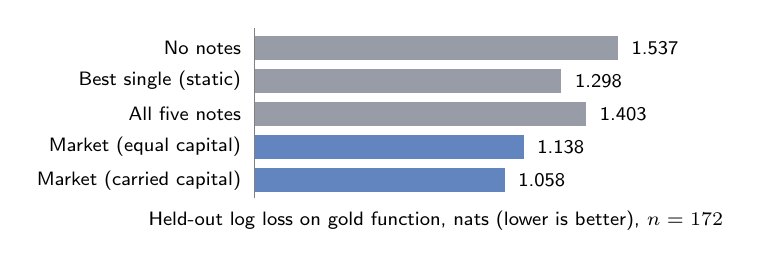
\begin{tikzpicture}[font=\sffamily\scriptsize]
\def\s{3.0}
\foreach \y/\name/\v/\c in {0/No notes/1.537/neutral, 1/Best single (static)/1.298/neutral, 2/All five notes/1.403/neutral, 3/Market (equal capital)/1.138/trade, 4/Market (carried capital)/1.058/trade} {
  \fill[\c!70] (0,-\y*0.42) rectangle (\v*\s,-\y*0.42-0.3);
  \node[anchor=east] at (-0.05,-\y*0.42-0.15) {\name};
  \node[anchor=west] at (\v*\s+0.05,-\y*0.42-0.15) {\v};
}
\draw[gray] (0,0.1) -- (0,-2.05);
\node[anchor=north] at (2.3,-2.1) {Held-out log loss on gold function, nats (lower is better), $n=172$};
\end{tikzpicture}
\caption{\textbf{MarketDebug.} Top: agents trade on private beliefs and reveal evidence; one settlement pays three separate ledgers. Bottom: on 210 held-out MarketBugs bugs, the five Gemma specialists trading in an LMSR market produce markedly better-calibrated forecasts than any single Gemma call, including one that sees all notes. Top-1 accuracy is unchanged (Table~\ref{tab:main}).}
\label{fig:teaser}
\end{figure}

\section{Related work}
\textbf{Agentic software engineering.} SWE-bench~\cite{swebench} and SWE-agent~\cite{sweagent} established repository-level repair with large API models. Agentless~\cite{agentless} showed that a fixed localize-then-repair pipeline is competitive. Fault localization remains the main bottleneck for small models~\cite{marketbugs}.
\textbf{Multi-agent aggregation.} Self-consistency~\cite{selfconsistency} and multi-agent debate~\cite{debate} combine samples from the same model. They pay no attention to which agent contributed what.
\textbf{Markets and information elicitation.} Proper scoring rules~\cite{gneiting} reward honest probabilities. The LMSR~\cite{hanson2003} turns scoring rules into an automated market maker with bounded subsidy $b\ln n$. Conitzer~\cite{conitzer2009} connects prediction markets, marginal information rewards and the Shapley value~\cite{shapley}. To our knowledge this is the first application of these mechanisms to coding agents.

\section{Method}\label{sec:method}
\textbf{Markets.} For each bug we open an $n$-outcome LMSR market over the retrieved candidate functions. The cost function is $C(\mathbf{q}) = b \ln \sum_i e^{q_i/b}$, and the price of outcome $i$ is $\mathrm{softmax}(\mathbf{q}/b)_i$. A share of outcome $i$ pays one credit if $i$ is the buggy function. The market opens at the no-notes Gemma forecast.

\textbf{Agents and trading.} Each agent holds capital (1{,}000 credits) and a belief $\mathbf{p}_a$. On its turn it moves the log-prices a fraction $\alpha\in[0,1]$ of the way toward its belief, $\mathbf{t}\propto \mathbf{p}^{1-\alpha}\mathbf{p}_a^{\alpha}$. It chooses the largest $\alpha$ whose cost stays within its per-turn budget (20\% of capital, split over three rounds). Shares are buy-only. A risk-neutral agent with unlimited capital would set $\alpha=1$. The budget turns the market into a capital-weighted logarithmic pool whose weights are \emph{earned}.

\textbf{Ledger 1: trading.} At settlement each agent receives its shares on the gold outcome. Trading P\&L is payout minus spend. Capital carries to the next bug, so agents that were right gain influence. This is the selection channel through which rewards change the behavior of a frozen LLM.

\textbf{Ledger 2: information.} Each revealed fact is posted to a timestamped board. A fact counts only if it was not already public, which prevents a copycat from splitting the original finder's credit. Let $v(S) = s(\mathbf{p}_S, x) - s(\mathbf{p}_\emptyset, x)$ for a proper scoring rule $s$ (log score here). Here $\mathbf{p}_S$ is the forecaster's output given only the facts of coalition $S$, and $x$ is the realized outcome. We implement three credit rules: marginal (score change in filing order), Shapley $\phi_i = \frac{1}{n!}\sum_\pi [v(P_i^\pi\cup\{i\}) - v(P_i^\pi)]$ (exact for $n\le 8$, permutation-sampled otherwise), and pivotal $v(N)-v(N\setminus\{i\})$. Shapley credit is budget-balanced and independent of reveal order. Pivotal credit generally is not. These are Conitzer-inspired. Their incentive guarantees rest on assumptions that LLM agents need not satisfy, so we treat them as hypotheses to test.

\textbf{Ledger 3: repair.} Every proposed patch gets a binary market ``will this patch pass?''. Patches are tested in descending price order up to a test budget, and the first passing patch is accepted. Its author receives a bounty, 30\% of which is shared among the original finders of the facts it cites. Root-cause markets resolve from the accepted patch's diff, which gives diagnostic questions a checkable answer.

\section{Experiments}\label{sec:exp}
\textbf{Data.} MarketBugs~\cite{marketbugs} contains single-function AST mutants that fail a test deterministically. We use the 30 development bugs with complete coalition tables (all 32 note subsets) and the 210 held-out bugs from seven repositories never used in development (attrs, boltons, dateutil, isodate, more-itertools, tomli, toolz). Each bug has 20 retrieved candidates. The gold function is in the pool for 172 of the 210 held-out bugs, and retrieval misses count as errors for every method.

\textbf{Agents.} The five specialists (trace, graph, spec, static, semantic) each write a note from a different view of the bug. Beliefs are the frozen Gemma~4 E4B-it probability-agent forecasts given only that specialist's note. They are read from the logits of 20 single-token labels and averaged in log space over two candidate orders. All forecasts are cached outputs of the pinned model revision \texttt{google/gemma-4-E4B-it@4ecc2ba}~\cite{marketbugs}. The market layer runs on a CPU in seconds.

\textbf{Methods.} \emph{No notes}; each \emph{single} specialist; \emph{all notes} (one Gemma call with all five notes, averaged over five note orders, the strongest prior baseline); an equal-weight \emph{log pool}; the \emph{market} with fresh equal capital per bug; and the \emph{market} with capital carried across bugs (dev first, then held-out). Market settings: $b=50$, 3 rounds, random turn order, seed 0.

\begin{table}[t]
\centering\small
\caption{Held-out results (210 bugs). Top-1 counts retrieval misses as errors. Log loss is on the gold function for the 172 bugs with gold in the pool.}
\label{tab:main}
\begin{tabular}{lcc}
\toprule
Method & Top-1 (\%) $\uparrow$ & Log loss (nats) $\downarrow$ \\
\midrule
No notes & 62.4 & 1.537 \\
Single: trace / graph / spec & 61.4 / 63.8 / 63.8 & 1.449 / 1.334 / 1.472 \\
Single: static / semantic & 66.2 / 63.3 & 1.298 / 1.450 \\
All five notes (one call) & 64.8 & 1.403 \\
Log pool, equal weights & 64.8 & 3.872 \\
\midrule
\textcolor{trade}{Market, fresh capital} & 63.3 & 1.138 \\
\textcolor{trade}{Market, capital from dev} & 64.3 & \textbf{1.058} \\
\textcolor{trade}{Market, carried capital from equal start} & 63.8 & 1.061 \\
\bottomrule
\end{tabular}
\end{table}

\textbf{Accuracy is unchanged.} The paired top-1 difference between the market with carried capital and the all-notes call is $-0.5$ pp. Its 95\% two-stage repository-cluster bootstrap CI is $[-4.8, +3.8]$ (10{,}000 replicates). The fresh-capital market gives $-1.4$ pp $[-5.2, +2.4]$. Like the prior pooling result~\cite{marketbugs}, specialists built from one small model mostly agree on the top candidate, so no aggregation rule moves accuracy much.

\textbf{Calibration improves substantially.} Log loss falls from 1.403 (all notes) and 1.298 (best single) to 1.058 nats (Table~\ref{tab:main}, Figure~\ref{fig:teaser}). The equal-weight log pool, which multiplies five overconfident forecasts, is badly overconfident (3.87 nats). The market avoids this because budgets bound how far any trader can move the price. On the 30 dev bugs the pattern is the same: the fresh-capital market matches all notes on top-1 (76.7\%) and lowers log loss from 1.379 to 1.198.

\textbf{Shapley credit tracks usefulness.} On dev, where all 32 coalitions were cached, exact Shapley values in nats per bug rank graph (0.173) far above semantic (0.066), static (0.053), trace (0.050) and spec (0.027). On held-out bugs only singletons and the full set are cached. There we use the approximation $\phi_i = v(\{i\}) + (v(N) - \sum_j v(\{j\}))/n$, which is exact when interactions appear only in the full coalition. It gives static (0.129) and graph (0.093) positive credit and the other three slightly negative credit. This agrees with Table~\ref{tab:main}, where static and graph are the best single specialists. Capital after the held-out run tells the same story: graph 535, static 310, trace 157, spec 136, semantic 10 credits.

\textbf{Every trader loses money.} Held-out trading P\&L is negative for all five agents ($-376$ to $-999$ credits). Gemma's single-note forecasts are overconfident, so agents overpay for their favourite candidates, and the market maker's bounded subsidy does not cover the loss. Trading P\&L alone is therefore a poor reward for these agents. The separate information ledger is what credits the useful specialists, which supports keeping the ledgers apart.

\section{Discussion and limitations}
The market layer is cheap and model-agnostic, and it gives better-calibrated localization forecasts. That matters for an agent that must decide which candidate to patch first, or when to stop and run tests. It does not increase accuracy here, because the specialists share one base model and are not independent. Several limitations apply. Our traders are frozen forecasts, not agents that choose what to investigate. The incentive channel tested is capital selection, not in-context or RL-trained response to rewards. Only seven held-out repositories bound the bootstrap. Held-out Shapley values use an approximation. Mutants are not natural bugs. The repair ledger and patch markets are implemented but were not run end-to-end with Gemma-generated patches before the deadline. The natural next steps are diverse specialists (different models, tools and starting files), agents that observe prices and balances in context, and RL fine-tuning of Gemma on the information-reward signal.

\section{Conclusion}
Paying agents for being right, for useful evidence, and for working fixes separately is easy to implement and auditable. On real Gemma~4 E4B forecasts it produces a calibrated group forecast and a credit assignment that identifies the useful specialists. Accuracy gains will require agents whose information actually differs.

\textbf{Reproducibility.} Code, cached forecasts and the benchmark script (\texttt{python -m marketdebug.gemma\_bench}) are in the project repository. The forecasts come from the public MarketBugs artifacts~\cite{marketbugs}.

\small
\begin{thebibliography}{99}
\bibitem{marketbugs} R.~Mondal et al. MarketBugs: What makes evidence aggregation reliable for small-model software debugging? \url{https://github.com/raunak2007/marketbugs}, 2026.
\bibitem{conitzer2009} V.~Conitzer. Prediction markets, mechanism design, and cooperative game theory. In \emph{UAI}, 2009.
\bibitem{hanson2003} R.~Hanson. Combinatorial information market design. \emph{Information Systems Frontiers}, 5(1):107--119, 2003.
\bibitem{shapley} L.~S. Shapley. A value for $n$-person games. In \emph{Contributions to the Theory of Games II}, 1953.
\bibitem{gneiting} T.~Gneiting and A.~E. Raftery. Strictly proper scoring rules, prediction, and estimation. \emph{JASA}, 102(477):359--378, 2007.
\bibitem{swebench} C.~E. Jimenez et al. SWE-bench: Can language models resolve real-world GitHub issues? In \emph{ICLR}, 2024.
\bibitem{sweagent} J.~Yang et al. SWE-agent: Agent-computer interfaces enable automated software engineering. In \emph{NeurIPS}, 2024.
\bibitem{agentless} C.~S. Xia et al. Agentless: Demystifying LLM-based software engineering agents. \emph{arXiv:2407.01489}, 2024.
\bibitem{selfconsistency} X.~Wang et al. Self-consistency improves chain of thought reasoning in language models. In \emph{ICLR}, 2023.
\bibitem{debate} Y.~Du et al. Improving factuality and reasoning in language models through multiagent debate. In \emph{ICML}, 2024.
\end{thebibliography}
\end{document}
